\documentclass[a4paper,10pt]{article}

\title{Bifurcation analysis of an ocean model}
\author{Leo Sok \& Harmen Stoppels}
\date{\today}
\usepackage{amsmath,amssymb}
\usepackage{enumitem}
\usepackage{pdfpages}
\usepackage{epstopdf}
\usepackage{graphicx}
\usepackage{subcaption}

\def\*#1{\mathbf{#1}}

\newcommand{\ra}[1]{\renewcommand{\arraystretch}{#1}}

\begin{document}
  \maketitle

  \begin{figure}[b!]
  \centerline{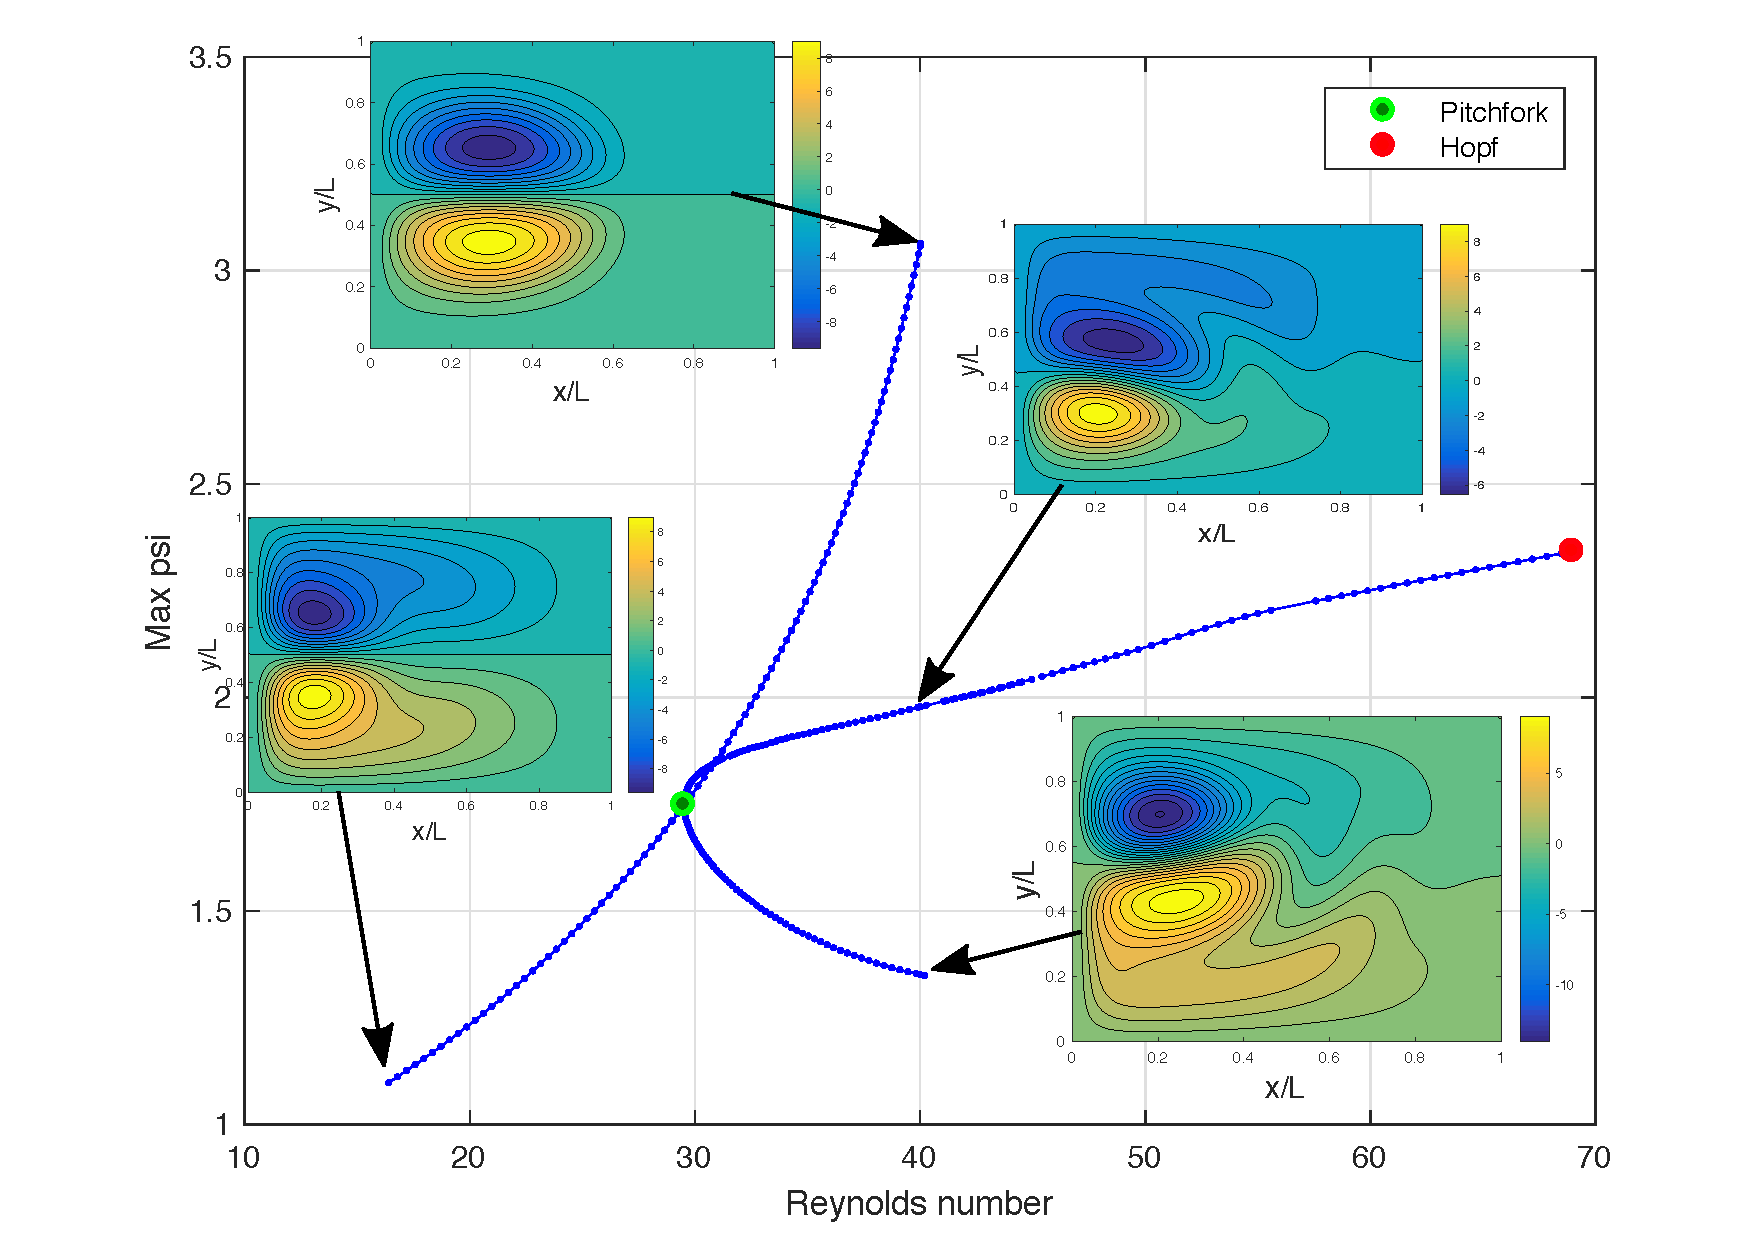
\includegraphics[width=1.3\textwidth]{images/bifurcatie_met_plots.pdf}}
  \caption{This bifurcation diagram gives an overview of the interesting points the ocean model. We see both a pitchfork and a Hopf bifurcation point. The subplots are the streamfunctions at the given parameters.}\label{fig:bifurcation_diagram}
  \end{figure}

  %!TEX root = ../report.tex
\section{Introduction}

We consider the PDE of the stream function $\psi = \psi(t, x, y):$
\begin{equation}\label{eq:pde}
\begin{aligned}
  \left(\frac{\partial}{\partial t} + u \frac{\partial}{\partial x} + v \frac{\partial}{\partial y}\right) \zeta + \beta \frac{\partial \psi}{\partial x} &= -\alpha \frac{\partial \tau_x}{\partial y} + \frac{1}{Re} \Delta \zeta & \text{in } [0, \infty) \times [0,1]^2, \\
  \zeta &= \Delta \psi & \text{in } [0, \infty) \times [0,1]^2, \\
  \psi = v &= 0 & \text{on } x = 0 \text{ and } x = 1, \\
  \psi = \zeta &= 0 & \text{on } y = 0 \text{ and } y = 1
\end{aligned}
\end{equation}
where $u = -\frac{\partial \psi}{\partial y}$ and $v = \frac{\partial \psi}{\partial x}$ and the wind-stress forcing is
\begin{equation}
  \tau_x(t, x, y) = \frac{- \eta}{2 \pi} \cos{2\pi y}.
 \label{eq:tau}
\end{equation}
We keep $\alpha = \beta = 1000$ fixed, and start with $Re = 16$ and $\eta = 0,$ such that the trivial solution $\psi = 0$ satisfies~\eqref{eq:pde}. Furthermore, we discretize~\eqref{eq:pde} in space on a $128\times128$ grid so that the PDE reduces to a system of ODEs.

\subsection{General continuation theory}
We're looking for equilibria of~\eqref{eq:pde} such that $\frac{\partial \zeta}{\partial t} = 0.$ Let $\*x$ denote the unknowns and $p$ denote the parameter we wish to change. We want to find $\*x$ such that $F(\*x, p) = 0,$ bla bla bla. 

\begin{enumerate}
  \item Parametrize $\Gamma(s) = (\*x(s), p(s)).$
  \item Find a starting point $\Gamma(s_0)$ s.t. $F(\Gamma(s_0)) = 0.$
  \item Compute $\dot\Gamma(s_0)$ (once, explicitly.)
  \item Repeat the predictor-corrector iteration until you reach a point of interest.
  \begin{description}
    \item[Predict:] For $s_{k+1} = s_k + \Delta s$ compute the guess $$(\*x^{(k+1)}, p^{(k+1)}) = \Gamma^{(k+1)} := \Gamma(s_k) + \Delta s * \dot\Gamma(s_k).$$
    \item[Correct:] Apply Newton's method in $\*x$ to $F(\*x, p^{(k+1)}) = 0$ with initial guess $\*x^{(k+1)}.$
  \end{description}
\end{enumerate}

  % %!TEX root = ../report.tex

% \begin{landscape}
% \thispagestyle{empty}
% \begin{figure}
% \centerline{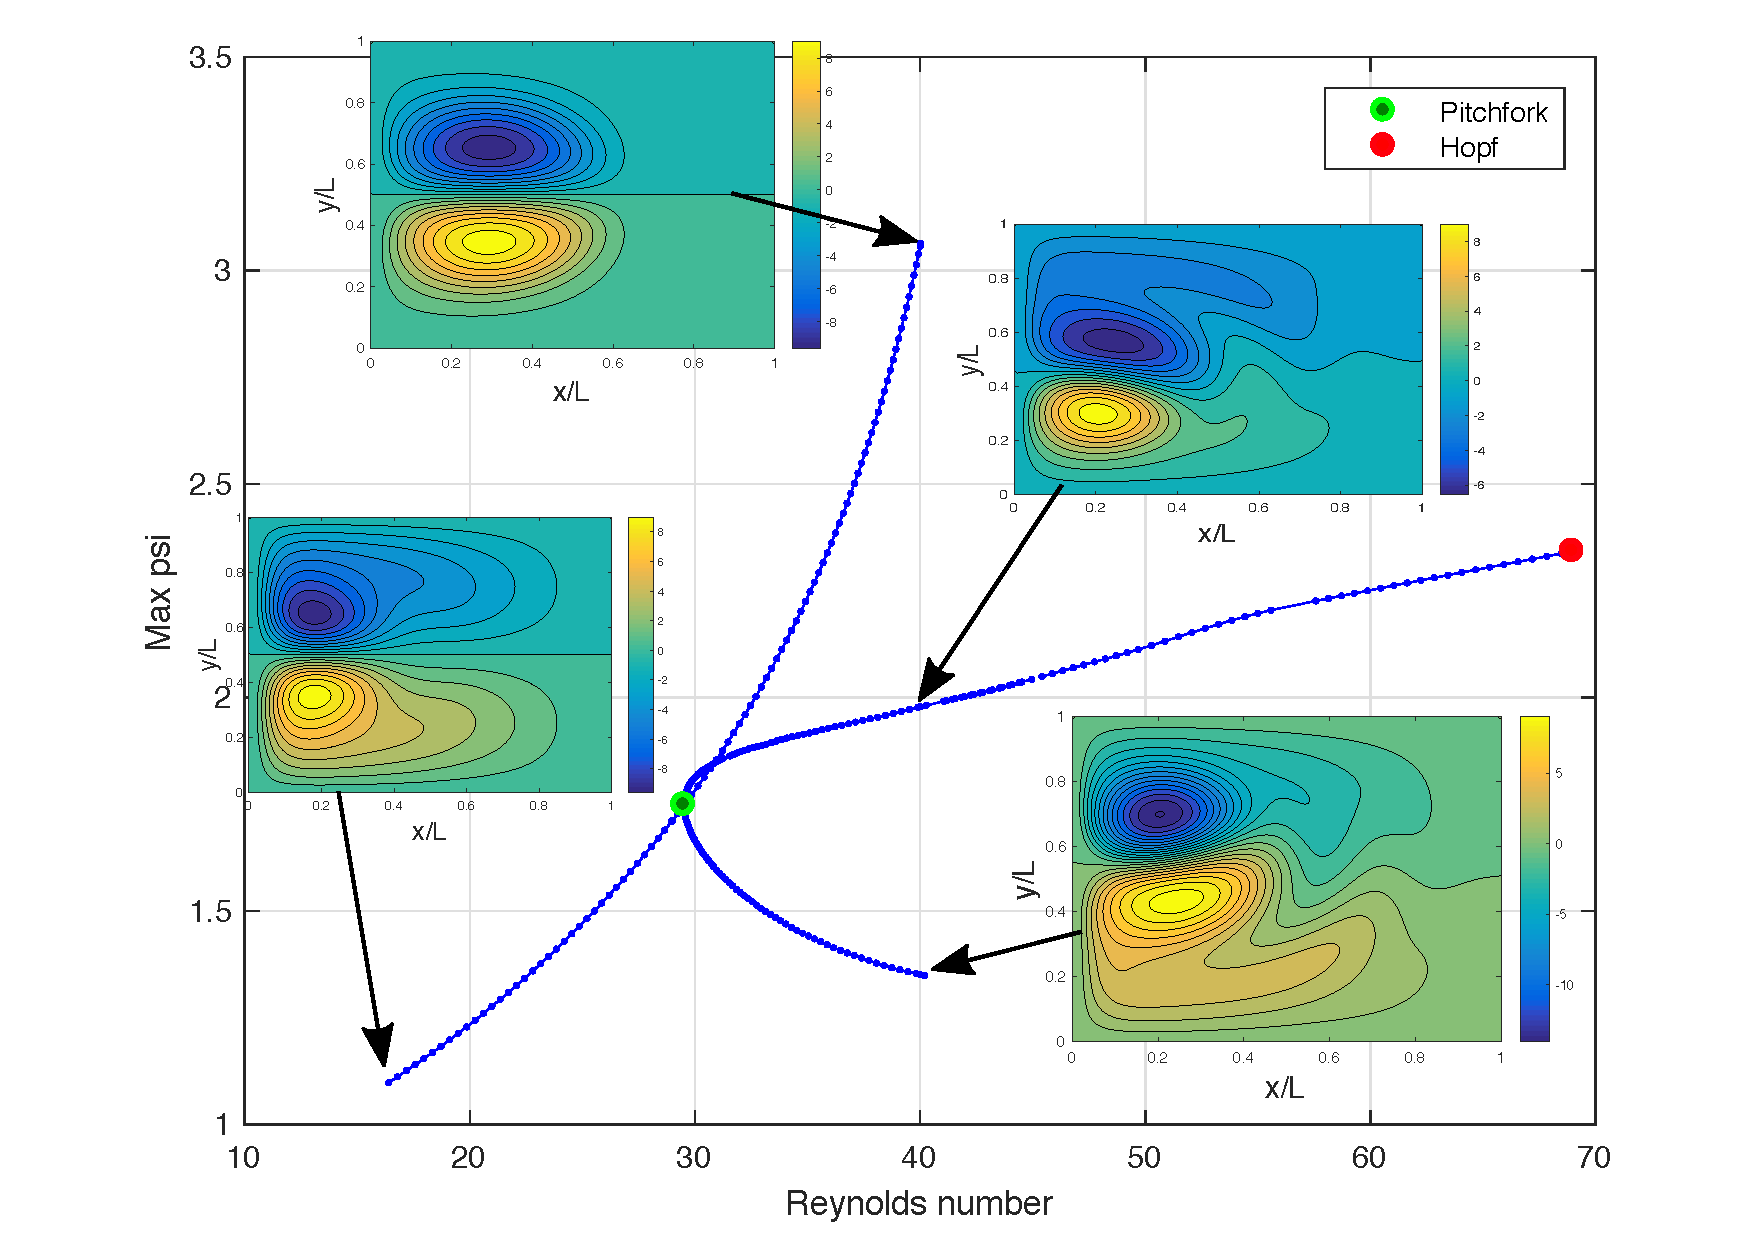
\includegraphics[width=0.9\textwidth]{images/bifurcatie_met_plots.pdf}}
% \caption{Bifurcation diagram}
% \end{figure}
% \end{landscape}


  %!TEX root = ../report.tex
\section{Spinup}

Starting from $\eta = 0$ with the trivial solution satisfying equation~\eqref{eq:pde}, we apply continuation in $\eta$ from $0$ to $1$ in steps of $\Delta s = 0.1$ and find a non-trivial solution at $Re = 16$ as shown in Figures~\ref{fig:question_a_psi} and~\ref{fig:question_a_zeta}.

\begin{figure}[h]
    \centering
    
    \caption{First non-trivial solutions after spin-up}\label{fig:question_a}
    \centerline{
    \begin{subfigure}[b]{0.6\textwidth}
        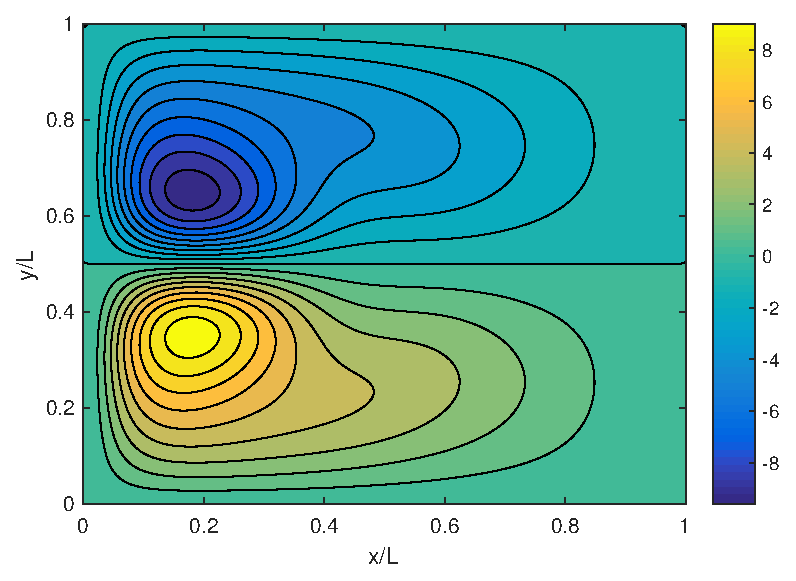
\includegraphics[width=\textwidth]{images/a_psi.eps}
        \caption{Streamfunction $\psi$ at $Re = 16$}
        \label{fig:question_a_psi}
    \end{subfigure}
    ~
    \begin{subfigure}[b]{0.6\textwidth}
        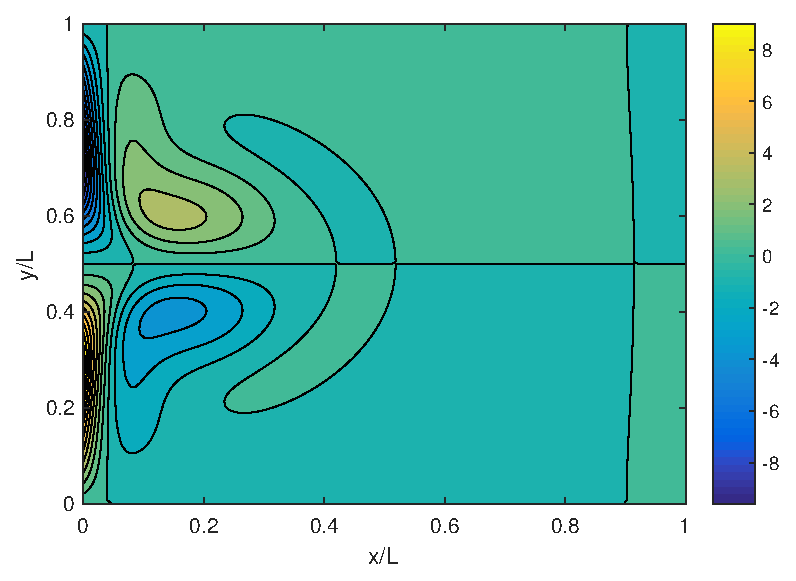
\includegraphics[width=\textwidth]{images/a_zeta.eps}
        \caption{$\zeta$ at $Re = 16$}
        \label{fig:question_a_zeta}
    \end{subfigure}
    }
\end{figure}

  %!TEX root = ../report.tex
\section{Preconditioning}

The iterative solver is $\textrm{CGSTAB}$ with $ILU$ as a preconditioner. The preconditioner has a single parameter $\epsilon$ which determines the drop tolerance in the incomplete decomposition. A value of $\epsilon = 0$ reduces to a full LU decomposition, which requires too much work and memory, and would make an iterative method superfluous. On the other hand, if $\epsilon = 1$, the preconditioner simply reduces to a diagonal matrix, which is cheap to apply, but maybe not as effective. Typically the optimal value for $\epsilon$ must be found experimentally. In our case it turns out $\epsilon \approx 10^{-6}$ is an optimal value in terms of CPU time spent on a single continuation step in $Re$ at $Re \approx 16$ and $\eta = 1$ (given the initial direction). See Figure~\ref{fig:optimal_epsilon} for reference.

% \begin{wrapfigure}{l}{0.25\textwidth}
\begin{figure}[h]
    \centering
    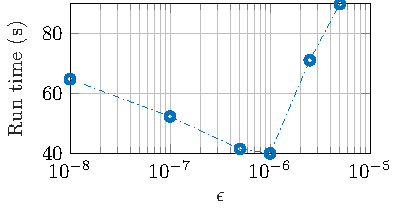
\includegraphics{images/droptol_epsilon.pdf}
    \caption{Finding the optimal drop tolerance paramter $\epsilon$ experimentally.}
    \label{fig:optimal_epsilon}
\end{figure}
% \end{wrapfigure}

  \section{Changing grid resolution}

\begin{figure}[h]
    \centering
    \caption{$\psi$ at $Re = 16$ for different grid sizes}\label{fig:grids}
    \centerline{
    \begin{subfigure}[b]{0.6\textwidth}
        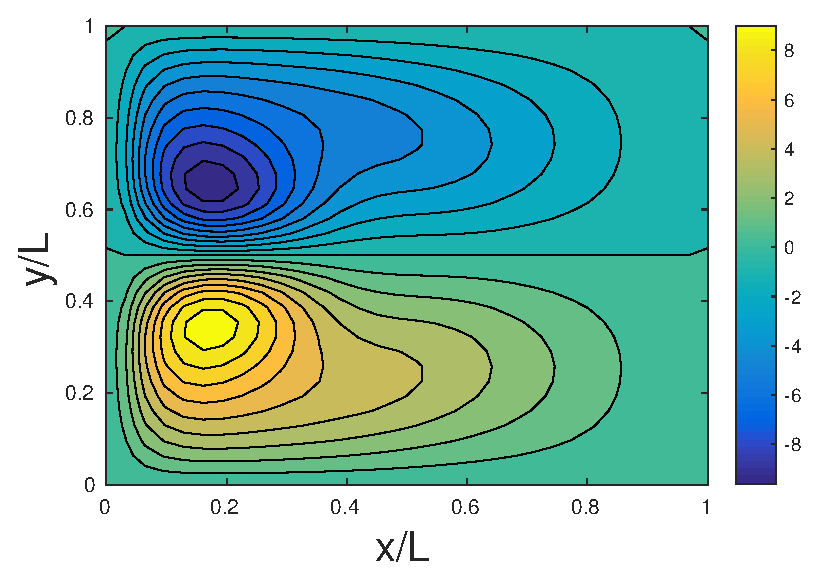
\includegraphics[width=\textwidth]{images/grid32.eps}
        \caption{$32\times 32$}
        \label{fig:nm32}
    \end{subfigure}
    ~
    \begin{subfigure}[b]{0.6\textwidth}
        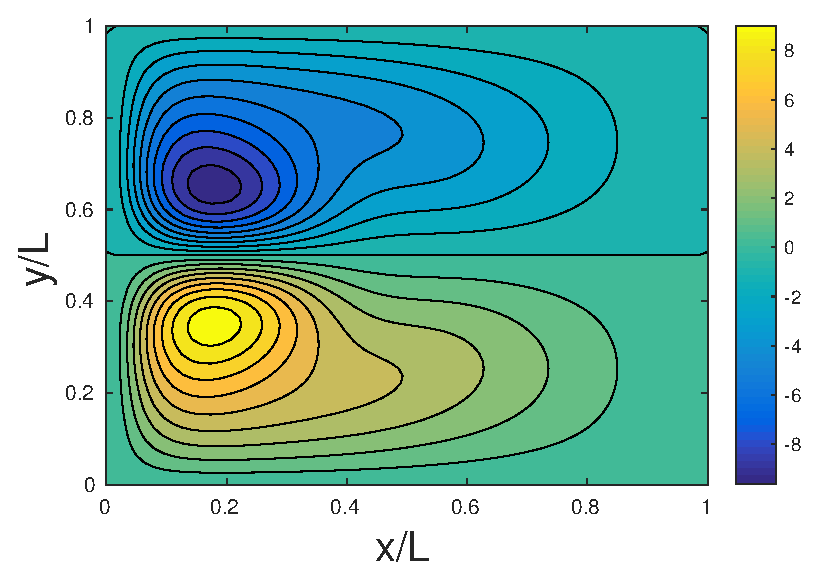
\includegraphics[width=\textwidth]{images/grid64.eps}
        \caption{$64\times 64$}
        \label{fig:nm64}
    \end{subfigure}
    }
    
    \begin{subfigure}[b]{0.6\textwidth}
        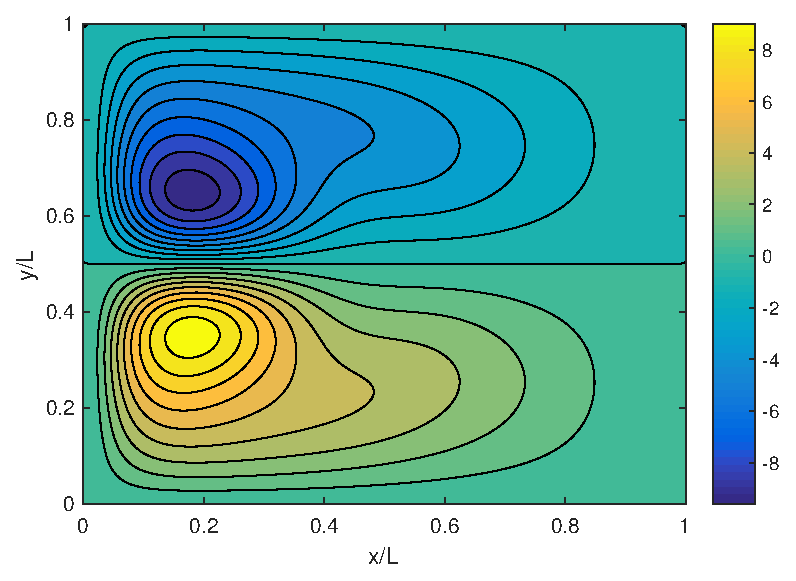
\includegraphics[width=\textwidth]{images/grid128.eps}
        \caption{$128\times 128$}
        \label{fig:nm128}
    \end{subfigure}
    
\end{figure}

\begin{figure}
	\includegraphics[width=\textwidth]{images/errors.pdf}
	\caption{Difference between values of the stream function for grid size $N\times N$ minus the value for grid size $N-32 \times N-32$}
	\label{fig:errors}
\end{figure}

In order to check whether the accuracy of the solutions in adequate, we changed the resolution of the model. We have determined a branch of steady states in $\eta$ for grid resolutions $32\times 32$, $64\times 64$, $96\times 96$, $128\times 128$ and $160\times 160$. In figure \ref{fig:grids}, the resulting streamfunctions are shown for three grid sizes. A quick look tells us that the shapes of the solutions are the same. For a more accurate approach, we have plotted in figure \ref{fig:errors} the difference between the value at three points of the streamfunction for different grid sizes (Diff). In these figure, the straight line ($\sim/N^2$) is a reference to determine whether the accuracy is second order. When we compare Diff with $\sim/N^2$, we see that the solution, for grid sizes around $128\times 128$ is approximately second order accurate. We can also see, that when we refine the grid to sizes larger than $128\times 128$, the error reduces only by a term of order $10^{-2}$, so we conclude that $128\times 128$ is small enough.

  %!TEX root = ../report.tex
\section{Internal (anti-)symmetry}

In this section, we will show the internal (anti-)symmetry of the PDE \eqref{eq:pde}, which means that a given steady state $$\psi(x, y),$$ where we drop $t$ since we are assuming steady states, produces another steady state solution $$-\psi(x, 1 - y).$$

This anti-symmetry can give rise to a pitchfork bifurcation. Clearly a solution itself can be anti-symmetric along $y = 1/2$ such that $\psi(x,y)=-\psi(x,1 - y)$ are identical solutions. This is the case at $Re=16.$ However, with different parameters we could have two different anti-symmetric solution $\psi(x,y) \neq -\psi(x,1 - y),$ which correspond to the ``upper'' and ``lower'' branch of the pitchfork bifurcation.

We will first show that if we have a steady state $\psi(x,y)$, then $-\psi(x,1-y)$ is also a steady state. Suppose we have found a steady state $\psi(x,y)$. Then, if we rewrite the PDE \ref{eq:pde}, we get
 \begin{equation}
   \frac{\partial}{\partial t}\zeta= - \underbrace{   u \frac{\partial\zeta}{\partial x}}_{=:\ref{eq:steady} a} +\underbrace{  v \frac{\partial\zeta}{\partial y}}_{=:\ref{eq:steady}b} - \beta \underbrace{\frac{\partial \psi}{\partial x} }_{=:\ref{eq:steady}c} - \alpha\underbrace{ \frac{\partial \tau_x}{\partial y}}_{=:\ref{eq:steady} d} +\frac{1}{Re}  \underbrace{\Delta \zeta}_{=:\ref{eq:steady}e}=0\label{eq:steady}
\end{equation}
 $$\zeta=\Delta \psi $$
Now we want to show that 
$$\bar{\psi}(x,y)=-\psi(x,\bar{y}) \text{ with }\bar{y}=1-y$$
is also a steady state.

So we want to show that, if \eqref{eq:steady} holds, 
 \begin{equation} \frac{\partial}{\partial t}\bar{\zeta}=- \underbrace{  \bar u \frac{\partial\bar{\zeta}}{\partial x}}_{=:\ref{eq:othersteady} a} +\underbrace{ \bar v \frac{\partial\bar{\zeta}}{\partial y}}_{=:\ref{eq:othersteady}b} -\beta \underbrace{ \frac{\partial \bar{\psi}}{\partial x} }_{=:\ref{eq:othersteady}c} -\alpha  \underbrace{\frac{\partial \bar \tau_x}{\partial y}}_{=:\ref{eq:othersteady}d} + \frac{1}{Re} \underbrace{\Delta \bar{\zeta}}_{=:\ref{eq:othersteady}e}=0 \label{eq:othersteady}
 \end{equation}
 $$\bar{\zeta}=\Delta \bar{\psi}$$ 
We will show this by showing that the parts (a, b, c, d, e) in Equation~\eqref{eq:othersteady} are minus the same part in Equation~\eqref{eq:steady}. Therefore we will first show that $-\bar{u}=-u$ and $\bar{v}=v$. 
 
\begin{equation}
-\bar u=\frac{\partial \bar{\psi}}{\partial y}(x,y)=-\frac{\partial \psi}{\partial \bar y}(x,\bar y)\frac{\partial \bar{y}}{\partial y}=\frac{\partial \psi}{\partial \bar y}(x,\bar y)=-u
\label{eq:ubar}
\end{equation}

\begin{equation}
\bar v=\frac{\partial \bar{\psi}}{\partial x}(x,y)=-\frac{\partial \psi}{\partial x}(x,\bar y)=-v \label{eq:vbar}
\end{equation}
Before further computations we will show that $\bar{\zeta}=-\zeta$.

\begin{align}
\bar{\zeta}(x,y) &= \Delta \bar{\psi}(x,y)
=\frac{\partial^2\bar{\psi}}{\partial x^2}(x, y)+\frac{\partial^2\bar{\psi}}{\partial \bar y^2}(x, y) \nonumber \\
&=-\frac{\partial^2\psi}{\partial x^2}(x,\bar y)-\frac{\partial^2\psi}{\partial \bar y^2}(x,\bar y)
=-\zeta(x,\bar y)\label{eq:zetabar}
\end{align}

With these, we will now show that Equation~\eqref{eq:othersteady} follows from Equation~\eqref{eq:steady}.
We start with part a of the equations. Using equations~\eqref{eq:ubar} and~\eqref{eq:zetabar},
\begin{equation}
\ref{eq:othersteady} a=\bar u\frac{\partial\bar{\zeta}}{\partial x} (x,y) =-u \frac{\partial\zeta}{\partial x} (x,\bar y)=-\ref{eq:steady}a
\end{equation}
Then part b, using equations \eqref{eq:vbar} and \eqref{eq:zetabar},
\begin{equation}
\ref{eq:othersteady}b=\bar{v}\frac{\partial\bar{\zeta}}{\partial y} (x,y) =-v \frac{\partial\zeta}{\partial \bar y} (x,\bar y)=-\ref{eq:steady}b
\end{equation}
Equality of the parts c follows immediately from equation \ref{eq:vbar}
$$\ref{eq:othersteady}c=\frac{\partial \bar{\psi}}{\partial x}=\bar{v}=-v=-\frac{\partial \psi}{\partial x}=-\ref{eq:steady}c$$
For part d, we have defined $\bar{\tau}_x(y)=\tau_x(\bar y)$, where we have dropped the indices $t$ and $x$, because $\tau$ does not depend on them. So we get
$$\ref{eq:othersteady}d=\frac{\partial \bar \tau_x}{\partial y}(y)=\frac{\partial \tau_x}{\partial \bar y}(\bar y)\frac{\partial y}{\partial \bar y}=-\frac{\partial \tau_x}{\partial \bar y}(\bar y)=-\ref{eq:steady}d$$
Finally we look at part e of the equations. Using Equation~\eqref{eq:zetabar}, we get
\begin{align}
\ref{eq:othersteady}e& =\Delta \bar{\zeta}(x,y)
=\frac{\partial^2\bar{\zeta}}{\partial x^2}(x, y)+\frac{\partial^2\bar{\zeta}}{\partial \bar y^2}(x, y) \\
&=-\frac{\partial^2\zeta}{\partial x^2}(x,\bar y)-\frac{\partial^2\zeta}{\partial \bar y^2}(x,\bar y)=-\Delta\zeta(x,\bar y)=-\ref{eq:steady} e
\end{align}
Combining this five parts of equations~\eqref{eq:othersteady} and~\eqref{eq:steady} shows us that
$$\frac{\partial}{\partial t}\bar{\zeta}=-\frac{\partial}{\partial t}\zeta=0$$ and thus is $\bar{\psi}$ a steady state, which gives us the internal anti-symmetry of the system that gives rise to the pitchfork bifurcation.




  
  %!TEX root = ../report.tex
\section{Pitchfork}

Next, we show how to detect the pitchfork, continue on a non-trivial branch, recover the other non-trivial branch and lastly find the exact location of the bifurcation point. When we speak about the {\em upper} and {\em lower} branch, we refer to the non-symmetric branches with largest and smallest $\psi_{max}$ as shown in the bifurcation diagram of Figure~\ref{fig:bifurcation_diagram}.

\subsection{Detection}
The cheapest way to continue on upper branch of the pitchfork is to break the anti-symmetry of the PDE temporarily. This is carried out by adding a non-symmetric forcing term to the equation controlled by a new parameter {\tt asym}, continuing only a tad in the new parameter, subsequently continuing in $Re$ past the pitchfork bifurcation point, and lastly restoring symmetry by bringing {\tt asym} back to 0. To be more precise, we replace the wind stress forcing term $\tau_x$ by
\begin{equation}
    \tau_x := -\eta \left( \frac{1 - \mathtt{asym}}{2 \pi} \cos(2\pi y) + \frac{\mathtt{asym}}{\pi} \cos(\pi y) \right)
\end{equation}
such that the corresponding term in the right-hand side of the PDE~\eqref{eq:pde} becomes
\begin{equation}
    -\frac{\partial \tau_x}{\partial y} = -\eta (1 - \mathtt{asym})\sin(2\pi y) + \mathtt{asym}\sin(\pi y)).
\end{equation}
This clearly breaks the anti-symmetry $\partial_y \tau_x(y) \neq -\partial_y \tau_x(1 - y).$ We add the parameter $\mathtt{asym}$ at $Re = 16$ and continue in $\mathtt{asym}$ for two steps of $\Delta s = 0.1.$ We then continue in $Re$ until $Re \approx 31.$ At this point it becomes clear we have passed the pitchfork bifurcation point, by judging the behaviour of the solution as shown in Figure~\ref{fig:pitch_detection}. If we look at $\psi_{max}$ as a function of $Re,$ we see interesting behaviour around $Re \approx 29,$ where it suddenly increases and then flattens. Also the effective step size in $Re$ decreases while $\Delta s$ is kept constant at $0.1$; this could mean that the solution changes more rapidly. Even more pronounced is the graph of $\psi_{max} + \psi_{min}$ where we not only see the small disturbance in symmetry around $Re = 16,$ but as well how it blows up past $Re = 29.$ Another way to detect the bifurcation point is to look at a specific point of the solution such as $\psi(\tfrac{1}{8}, \tfrac{1}{8})$ or $\psi(\tfrac{3}{8}, \tfrac{3}{8})$ where a qualitative change in behaviour appears after $Re = 29.$

At $Re \approx 31$, we bring back $\texttt{asym}$ to $0.$ Next we continue to $Re = 40$ at which point we obtain the solution as plotted in Figure~\ref{fig:question_e}. Now that we are on a branch of non-symmetric steady states, we can easily get on its anti-symmetric counterpart (the lower branch) by continuing backwards in $Re$ from $Re = 40$ to $Re_p$ and then all the way to $Re = 40$ again. This is done by setting $\Delta s = -1.$ We plot the solution in Figure~\ref{fig:question_e_lower}. Although it is not immediately clear from the plot, we verified in Matlab the lower branch is indeed anti-symmetric around $y = 0.5$ compared with the upper branch.

\begin{figure}[p]
    \centering
    \caption{Detection of the pitchfork.}
    \label{fig:pitch_detection}
    \centerline{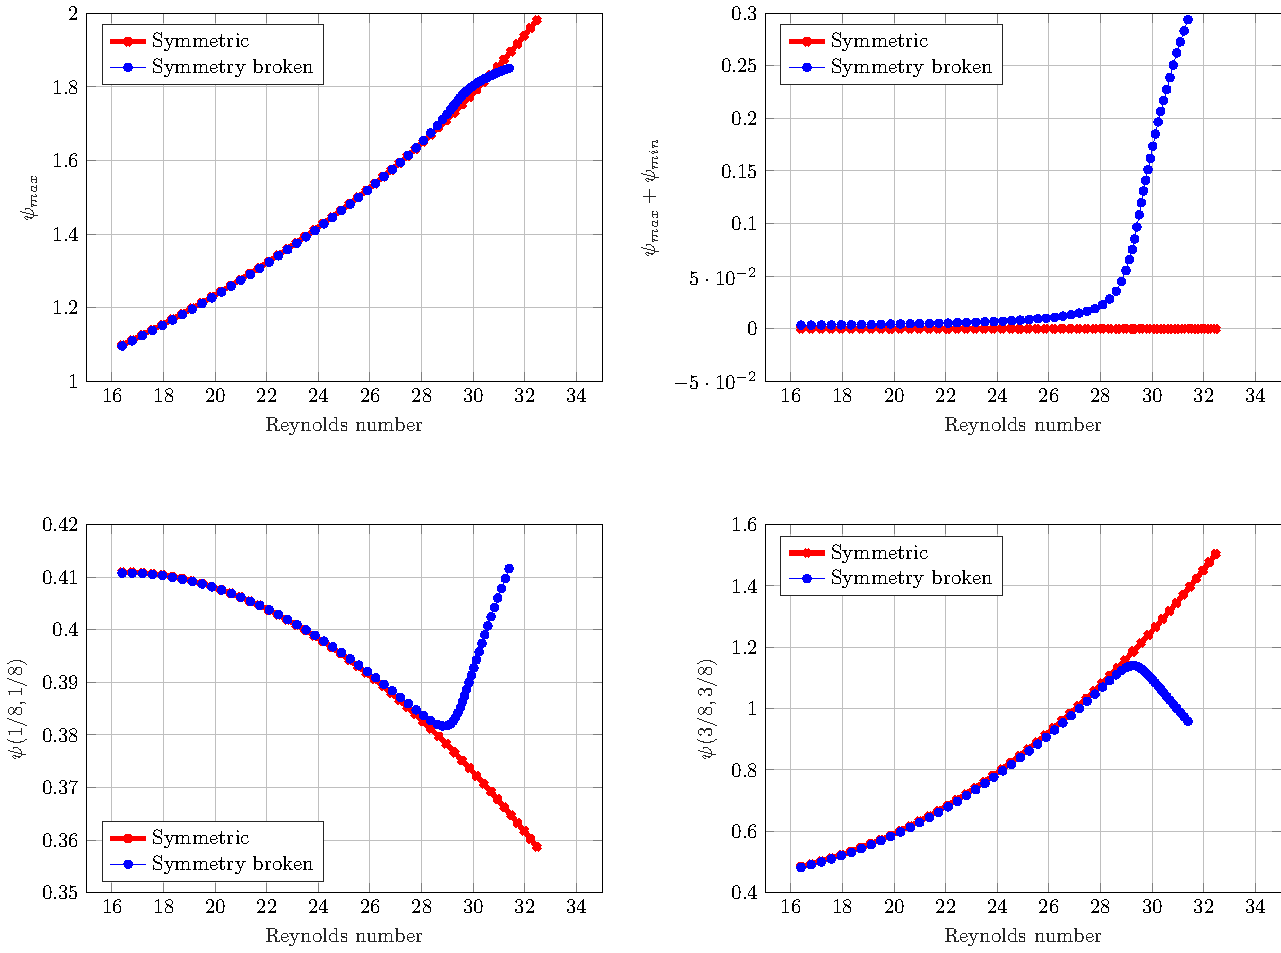
\includegraphics[width=1.3\textwidth]{images/pitch_detection.pdf}}
\end{figure}

\begin{figure}[p]
    \centering
    \caption{Solutions on the upper branch of the pitchfork}\label{fig:question_e}
    \centerline{
    \begin{subfigure}[b]{0.6\textwidth}
        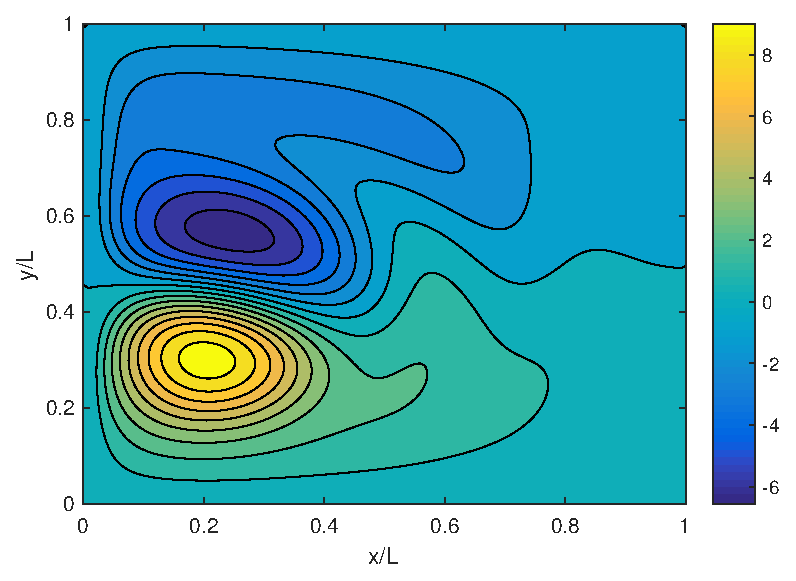
\includegraphics[width=\textwidth]{images/e_psi.eps}
        \caption{Streamfunction $\psi$ at $Re = 40$}
        \label{fig:question_e_psi}
    \end{subfigure}
    ~
    \begin{subfigure}[b]{0.6\textwidth}
        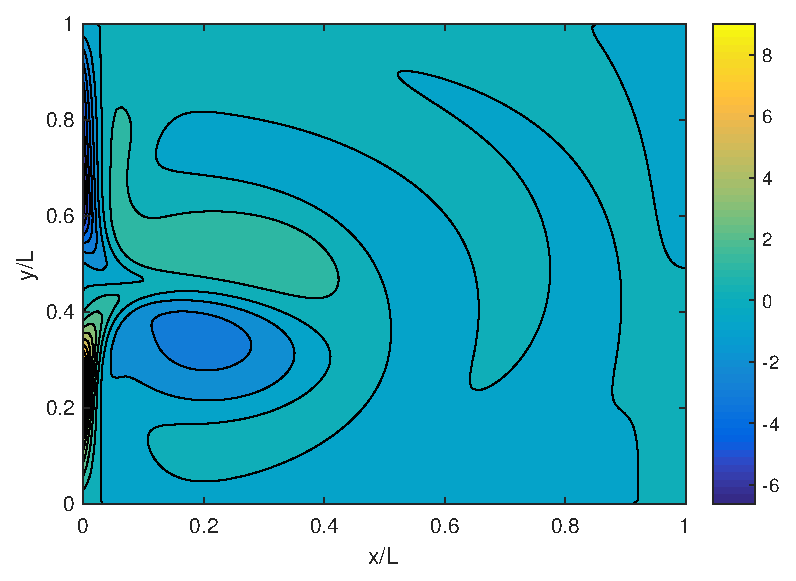
\includegraphics[width=\textwidth]{images/e_zeta.eps}
        \caption{$\zeta$ at $Re = 40$}
        \label{fig:question_e_zeta}
    \end{subfigure}
    }
\end{figure}


\begin{figure}[p]
    \centering
    \caption{Solutions on the lower branch of the pitchfork}\label{fig:question_e_lower}
    \centerline{
    \begin{subfigure}[b]{0.6\textwidth}
        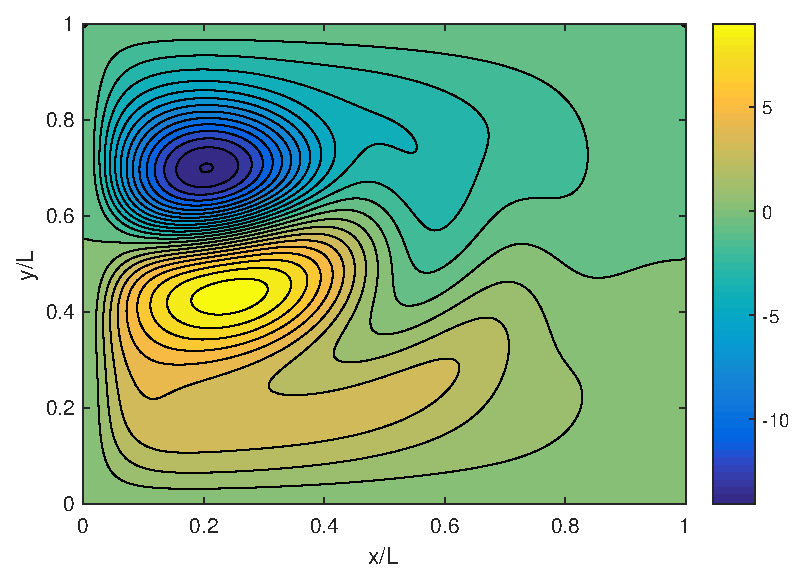
\includegraphics[width=\textwidth]{images/e_psi_lower.eps}
        \caption{Streamfunction $\psi$ at $Re = 40$}
        \label{fig:question_e_psi_lower}
    \end{subfigure}
    ~
    \begin{subfigure}[b]{0.6\textwidth}
        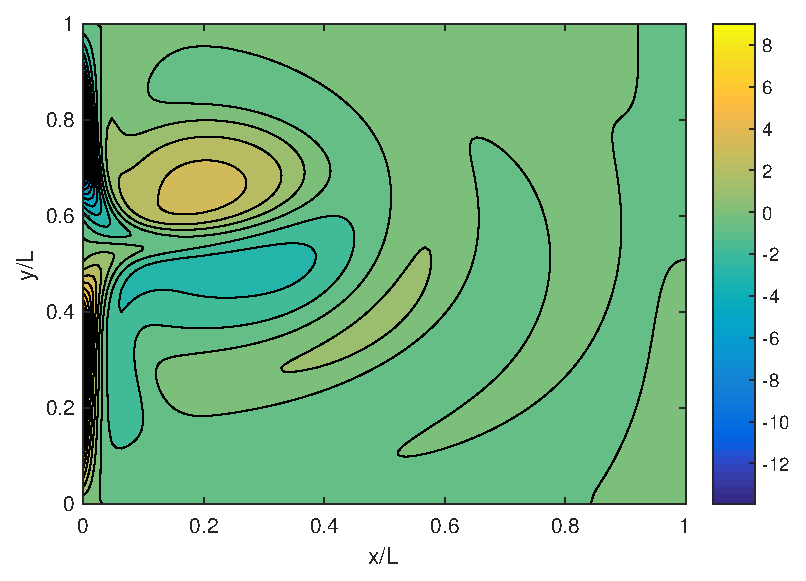
\includegraphics[width=\textwidth]{images/e_zeta_lower.eps}
        \caption{$\zeta$ at $Re = 40$}
        \label{fig:question_e_zeta_lower}
    \end{subfigure}
    }
\end{figure}

\begin{figure}[p]
    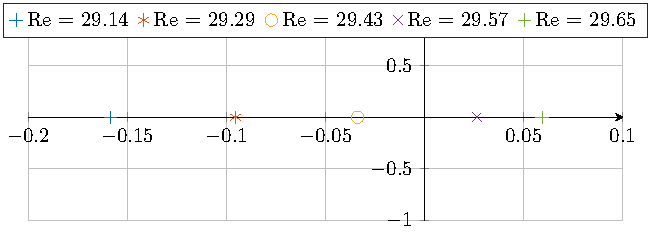
\includegraphics[width=\textwidth]{images/eigenvalues.pdf}
    \caption{An eigenvalue becomes positive after increasing the Reynolds number slightly}
    \label{fig:eigenvaluespitch}
\end{figure}

\newpage

\subsection{Finding its location and type}
In dynamical systems, the most fruitful way to assess non-linear systems is to look at their linearized approximation around an equilibrium. Via the Hartman-Grobman theorem the behaviour of the linearized system is under very mild conditions locally topologically equivalent to the non-linear system. Since we are always moving over an equilibrium, we can inspect the linearization $\*{\tilde u}$ of~\eqref{eq:ode} which is simply

\begin{equation}
    M\frac{d \*{\tilde u} }{d t} := DF_{\*u}\*{\tilde{u}}.
\end{equation}
To find the exact location of the pitchfork bifurcation and to inspect stability of the system, we can hence look at the generalized eigenvalue problem
\begin{equation}\label{eq:eigs}
    DF_{\*u}(\*u^*)x = \lambda M x
\end{equation}
where $\*u^*$ is a given equilibrium of the ODE~\eqref{eq:ode}.

To solve the generalized eigenvalue problem~\eqref{eq:eigs}, we use an eigenvalue solver (JDQZ) with a real target $\tau$ near the origin. This way we can detect a change of sign in the eigenvalues, and use the secant process to find exactly at which Reynolds number the pitchfork occurs. In Figure~\ref{fig:eigenvaluespitch} we show how the eigenvalue closest to the origin moves past the imaginary axis. It turns out that the ``exact'' location of the pitchfork is at $Re_p \approx 29.5112$.

Lastly, we use the eigenvalue solver to compute some eigenvalues on all branches away from the pitchfork and check the sign of the real part. It turns out that the pitchfork consists of three stable parts and one non-stable part, which fits in the category of {\em supercritical} pitchforks. 




  %!TEX root = ../report.tex
\section{Hopf bifurcation}

Continuing on the upper branch of the pitchfork, we compute (at most) 6 of the eigenvalues closest to the origin after a few steps in $Re.$ After a while we find that a conjugate eigenpair crosses the imaginary axis, which indicates a Hopf bifurcation is nearby. The movement of the eigenvalues is visualized in Figure~\ref{fig:eigenpair_crossing_imag}.

\begin{figure}[h]
  \centerline{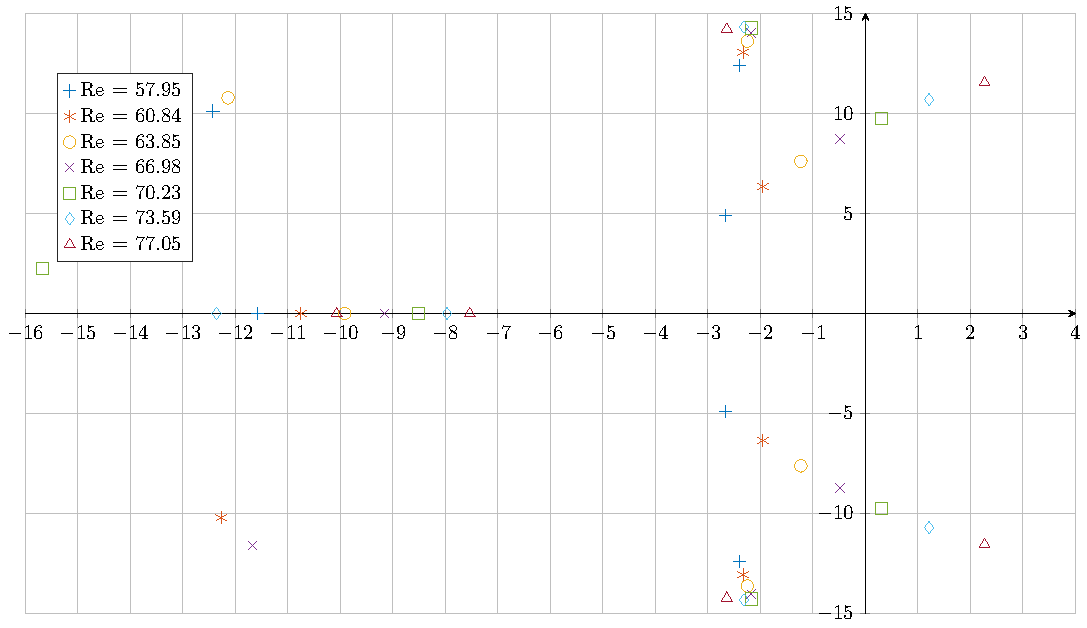
\includegraphics{images/eigenwaarden_hopf.pdf}}
  \caption{A conjugate eigenpair crossing the imaginary axis.}
  \label{fig:eigenpair_crossing_imag}
\end{figure}

We apply the secant procedure to compute the value of $Re$ where the first eigenvalue $\lambda$ is completely imaginary, i.e. $\Re(\lambda) = 0.$ We find that the Hopf bifurcation is located at $Re_H \approx 68.9781.$ The conjugate eigenpair is $$\lambda_\pm \approx \pm 9.372i.$$

Lastly we are interested in the corresponding eigenvectors. In fact they consist of two parts, since there are two discretized unknowns $\psi$ and $\zeta.$ The idea is to reconsider the eigenvalue problem of Equation~\eqref{eq:eigs} and interpret the Jacobian as being of the form
\begin{equation}
    DF_{\*u} = [DF_{\*\psi}, DF_{\*\zeta}]
\end{equation}
so that the first part of an eigenvector corresponds to the eigenfunction of $\psi$ and the second half of it corresponds to the eigenfunction of $\zeta.$ Also, we have both a real and an imaginary part of the eigenfunction. In Figure~\ref{fig:eigenfunction} we have plotted the ones corresponding to $\lambda_+.$ Note that the eigenfunction of $\lambda_-$ is identical up to a sign flip in the complex part.

\begin{figure}[h]
    \centering
    \caption{Eigenfunctions corresponding to $\lambda \approx 9.372i$.}\label{fig:eigenfunction}
    \centerline{
    \begin{subfigure}[b]{0.6\textwidth}
        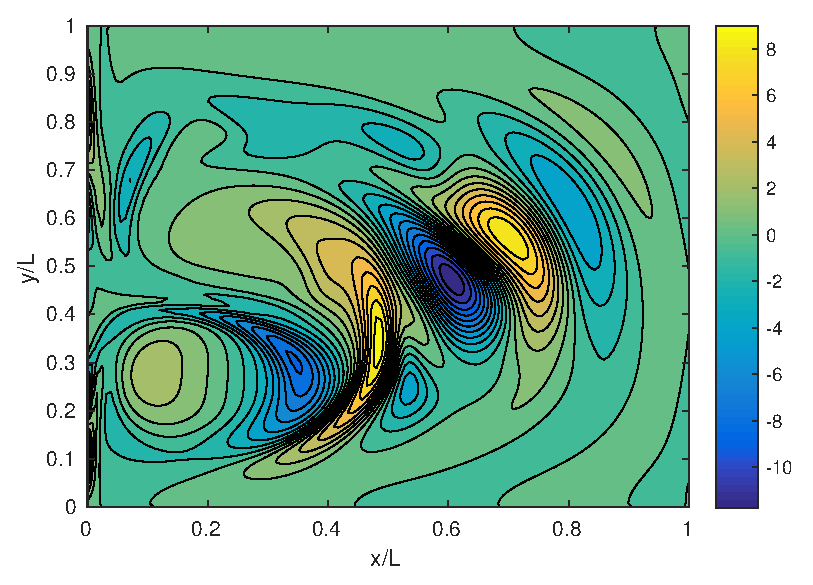
\includegraphics[width=\textwidth]{images/eigenvector_hop_1_2.eps}
        \caption{Real part corresponding to $\psi$}
        \label{fig:real_psi}
    \end{subfigure}
    ~
    \begin{subfigure}[b]{0.6\textwidth}
        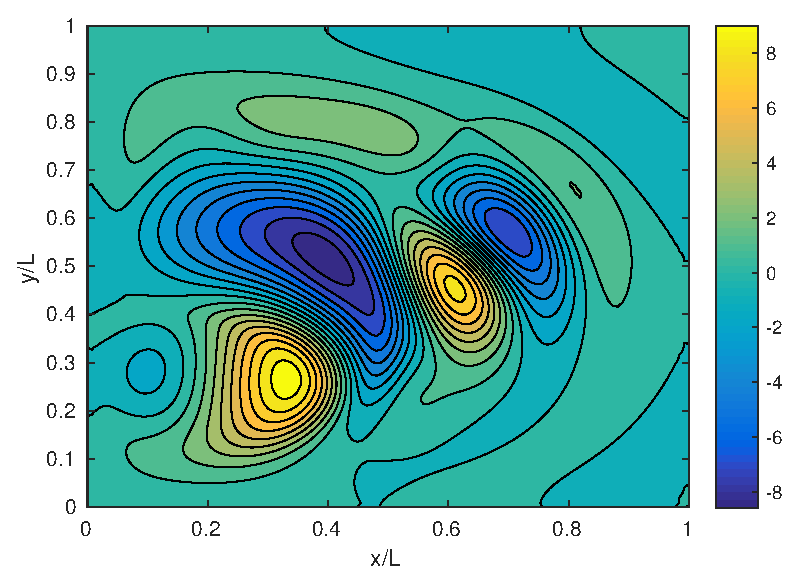
\includegraphics[width=\textwidth]{images/eigenvector_hop_2_2.eps}
        \caption{Real part corresponding to $\zeta$}
        \label{fig:real_zeta}
    \end{subfigure}
    }
    \centerline{
    \begin{subfigure}[b]{0.6\textwidth}
        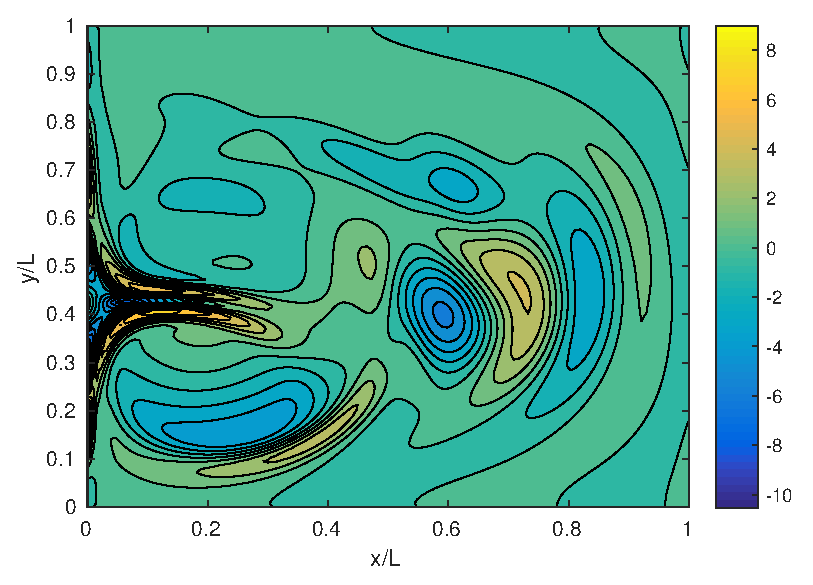
\includegraphics[width=\textwidth]{images/eigenvector_hop_1_3.eps}
        \caption{Imaginary part corresponding to $\psi$}
        \label{fig:imag_psi}
    \end{subfigure}
    ~
    \begin{subfigure}[b]{0.6\textwidth}
        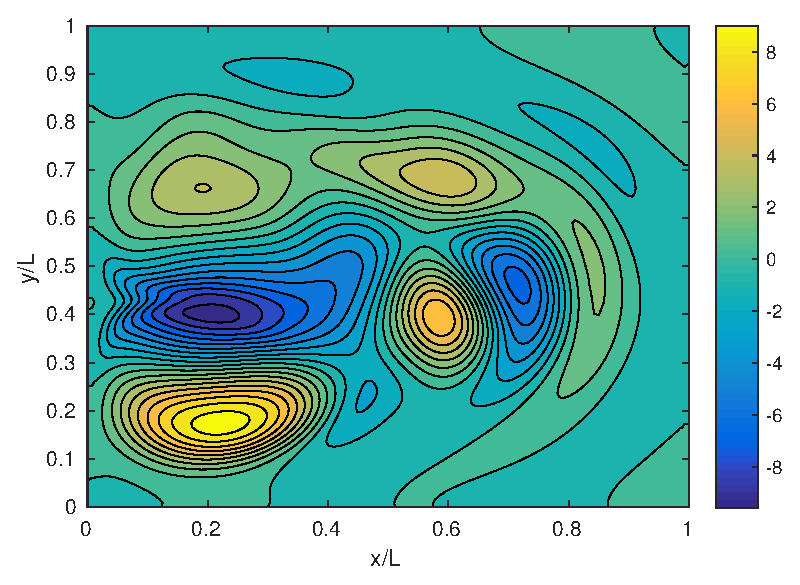
\includegraphics[width=\textwidth]{images/eigenvector_hop_2_3.eps}
        \caption{Imaginary part corresponding to $\zeta$}
        \label{fig:imag_zeta}
    \end{subfigure}
    }
\end{figure}
  
  \section{Conclusion}
We have looked at the steady states of the homogeneous wind-driven ocean circulation. We started with a trivial steady state with no wind-stress forcing and Reynolds number 16. From this steady state, we used a pseudo-arclength continuation in the wind forcing till we had full wind forcing. We found a steady state for which the streamfunction was symmetric. From this steady state, we applied a continuation in the Reynolds number to find a pitchfork bifurcation. This bifurcation appeared to be at $Re_p=29.5112$. In order to find the branches of asymmetric solutions, we started again at the steady state for $Re=16$. We broke the symmetry of the pitchfork by adding a non-symmetric forcing term. We applied a continuation in Re in this asymmetric system till we passed the bifurcation point. When we where at $Re\approx 31$, we went back to the original symmetric forcing system. So we and up on one of the branches of asymmetric solution. We used again the pseudo-arclength continuation, but now backwards in Re, following the branch through the bifurcation point and we found the other asymmetric branch.

After we found the pitchfork bifurcation, we also tried to find a Hopf-bifurcation. We started at the upper asymmetric branch of the pitchfork. The Hopf-bifurcation can only be detected by looking at the eigenvalues. So we applied a continuation in Re again, but at each step, we computed the eigenvalues and found that at $Re_H=68.9781$ a conjugate eigenpair crosses the imaginary axis and thus is there a Hopf bifurcation.
\end{document}